\documentclass{article}

\usepackage{ctex}
\usepackage{listings}
\usepackage[framed,numbered,autolinebreaks,useliterate]{mcode}
\usepackage{geometry}
\usepackage{multirow}
\usepackage{graphicx}
\usepackage{amsmath}
\usepackage{float}
\geometry{a4paper, scale=0.8}

\title{数学实验实验报告}
\author{ZhaohengLi 2017050025\\cainetatum@foxmail.com\\15801206130}

\begin{document}
\maketitle
\section{实验目的}
\begin{itemize}
	\item{掌握使用 LINGO 解线性和非线性规划的方法;}
	\item{通过求解实际问题,学会建立实际问题的线性和非线性规划模型。}
\end{itemize}


\section{CH8-T10 污水处理}

\subsection{模型建立}
设工厂总个数为 n,对应居民区总数也为 n,设每个居民区上游水流量为 $F_i$,下游水流 量为 $T_i$,上游污水浓度为 $U_i$,下游污水浓度为 $D_i$,从第 i 个居民区到第 i + 1 个居民区中 间段江水的自净系数为 $c_i$。第 i 个工厂的排水量为 $P+i$,处理前污水浓度为 $b_i$,处理过后的污 水浓度为 $d_i$,处理系数为 $e_i$。则可以写出如下等式$(i = 1, 2,\cdots,n)$:

$$F_i=T_{i-1},\quad T_i=F_i+P_i$$

$$U_i=(1-c_{i-1})D_{i-1}$$

$$D_i=\frac{F_iU_i+P_id_i}{F_i+P_i}$$

$$F_1=L_0\quad U_1=a_0$$

其中$L_0,a_0$为江水初始的流量和污水浓度。

为了满足实际污水处理情况,还需给出:

$$b_i\geq d_i,\quad i=1,2,\cdots,n$$

江面上所有地段水污染指数最高值和所有居民点上游水污染指数的最高值分别为:

$$maxD_i, maxU_i$$

如果给出最高值的限制 $\epsilon$,则上述条件可以扩展为 n 个限制(这一步转换是等价的):

$$D_i \leq \epsilon, \quad i=1,2,\cdots,n$$

或者

$$U_i \leq \epsilon, \quad i=1,2,\cdots,n$$


实际上,建立上述模型以及得出最高值的相关结论是基于对模型的一定假设和近似的,
具体对于模型的假设如下:

\begin{itemize}
	\item{假设污水产生的根源仅仅在于工厂;}
	\item{假设工厂 i 和居民区 i 在江水对岸,及工厂 i 的上游也是居民区 i 的上游,工厂 i 的下 游也是居民区 i 的下游;}
	\item{假设工厂在上游和下游的交界处瞬间将污水处理完成,且排出的污水和江水瞬间混合;}
	\item{假设在工厂处理污水的时候,不改变污水的流量。}
\end{itemize}

最后,处理污水总共需要花费的费用为:

$$\theta = \sum^n_{i=1}e_iP_i(b_i-d_i)$$

在处理具体问题的时候,由于上述变量大多为已知,带入具体数值即可,所要优化的变 量只有 $d_i$,可以近似成线性规划问题求解。


\subsection{算法设计}

根据上述模型分析可知,所有约束均为线性不等式,目标函数也为线性,符合线性规划 的一般形式,因此使用 LINGO 的 Linear Programming 功能直接进行求解即可。

最小化江面所有地段水污染的模型为:
\begin{lstlisting}
model:
title CH8-T10-1;

sets:
nd/1..3/:b,d,P;
endsets

data:
b=100,60,50;
enddata

min=5*@sum(nd:b-d);

P(1)=(1000*0.8+5*d(1))/1005;
P(2)=(1000*0.9*P(1)+5*d(2))/1010;
P(3)=(1000*0.6*P(2)+5*d(3))/1015;


P(1)<1;
P(2)<1;
P(3)<1;

b(1)>d(1);
b(2)>d(2);
b(3)>d(3);

end
\end{lstlisting}


最小化居民点上游的污水浓度模型为:
\begin{lstlisting}
model:
title CH8-T10-2;

sets:
nd/1..3/:b,d,P;
endsets

data:
b=100,60,50;
enddata

min=5*@sum(nd:b-d);

P(1)=(1000*0.8+5*d(1))/1005;
P(2)=(1000*0.9*P(1)+5*d(2))/1010;
P(3)=(1000*0.6*P(2)+5*d(3))/1015;

0.9*P(1)<1;
0.6*P(2)<1;

b(1)>d(1);
b(2)>d(2);
b(3)>d(3);

end
\end{lstlisting}


\subsection{分析和结论}

\subsubsection{计算结果}
最小化江面所有地段水污染的模型计算结果为:

\begin{figure}[H]
    \centering
    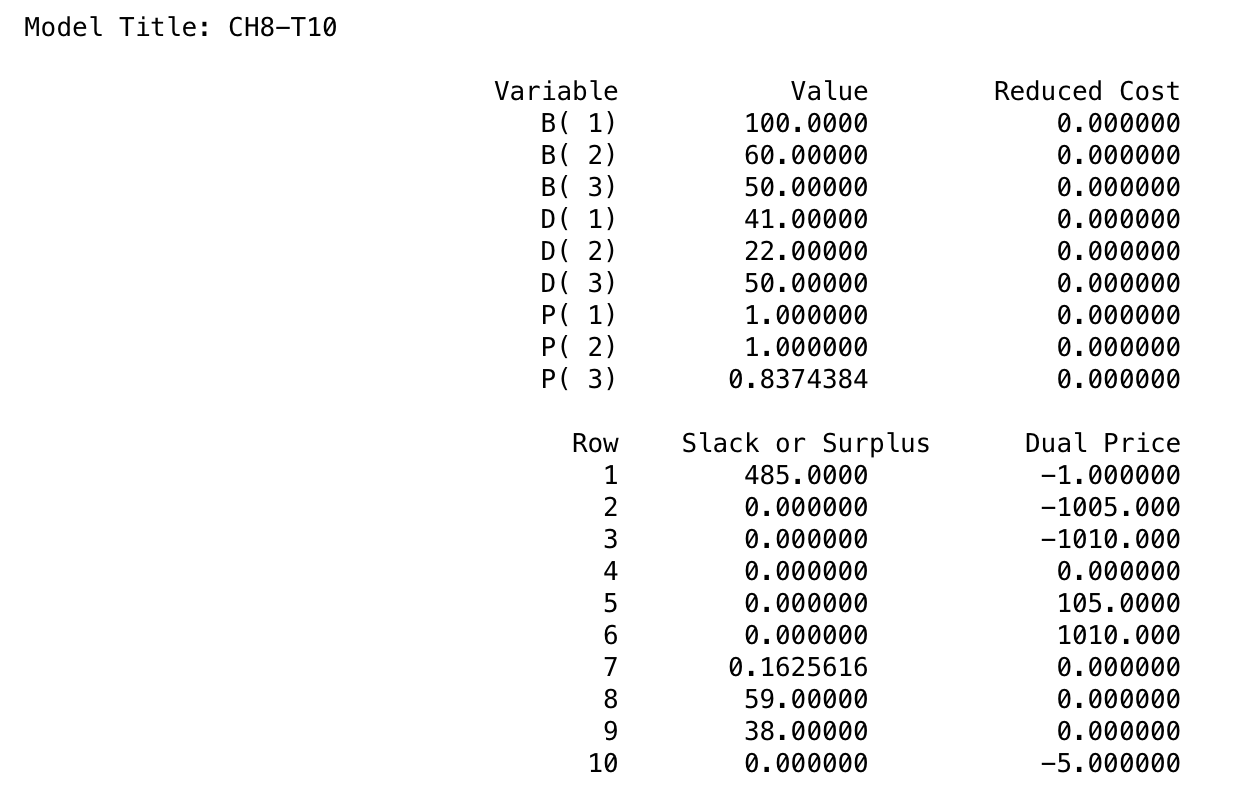
\includegraphics[width=0.8\textwidth]{pic1.png}
\end{figure}


可以看到,当限制江面所有地段水质的时候,模型求解变量的最优值为:


$$d_1=41.0,d_2=22.0,d_3=50.0$$

对应的减少费用均为 0,代表他们均为基变量。实际上,对于本小问,对应的约束矩阵 是满秩的。

最少费用为 485 万元。

最小化居民点上游的污水浓度模型计算结果为:

\begin{figure}[H]
    \centering
    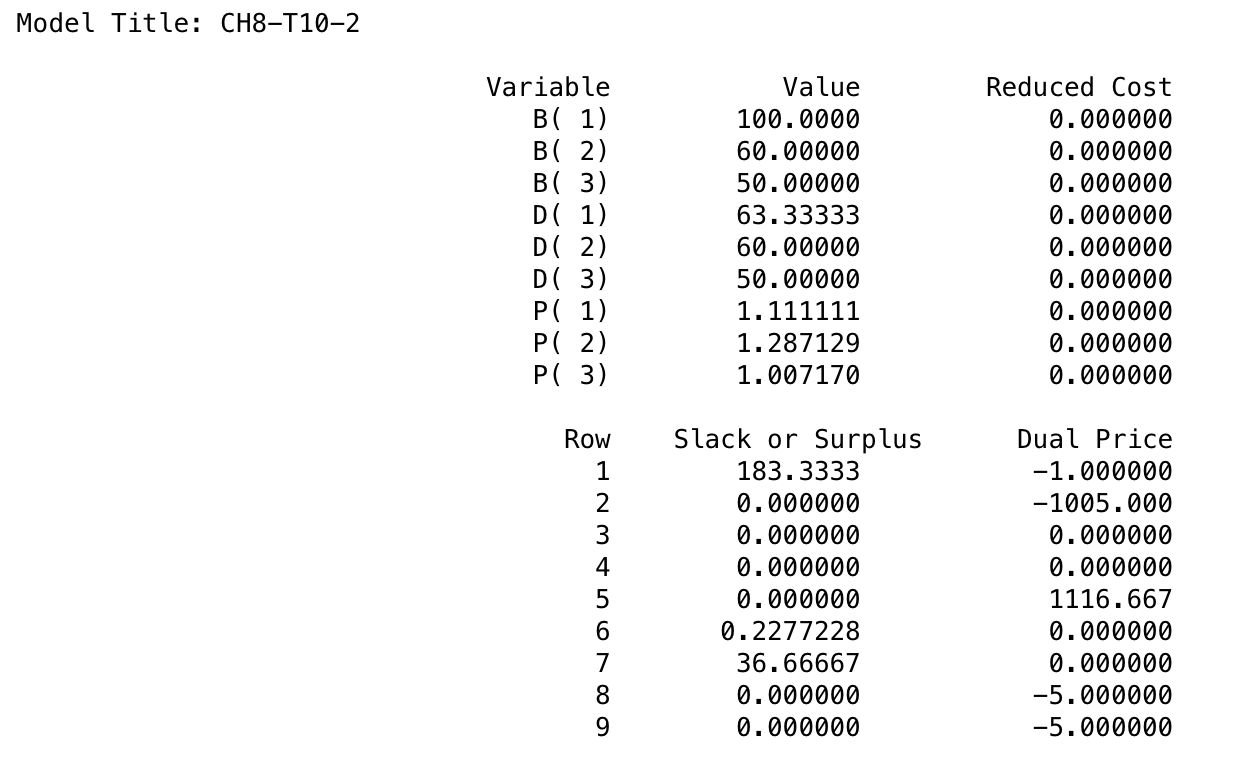
\includegraphics[width=0.8\textwidth]{pic2.png}
\end{figure}

可以看到,当限制居民点上游水质的时候,模型求解变量的最优值为:
$$d_1=63.3,d_2=60.0,d_3=50.0$$

对应的减少费用均为 0,代表他们均为基变量。
最少费用为 183.33 万元。

\subsubsection{结果分析}

对比两种模型,仅处理居民上游点水质的时候,费用明显减少。实际上,在给定 的假设下,限制所有地段水质等价于既处理居民点上游水质、又处理居民点下游的水质。第二种方案充分受益于河水的自净机制,如果河水的自净系数接近1的话,两种方案所需的花费差距将大大减小。

\subsubsection{结论}

当限制江面所有地段水质的时候,最少需要花费 485 万元;当限制居民点上游 水质的时候,最少需要花费 183.33 万元。


\section{CH9-T4 液体混合}

\subsection{模型建立}
首先我们对模型中所涉及到的参量进行描述。

假设购买原料甲 a 吨,原料乙 b 吨,原料丙 c 吨。

甲乙的混合物用于生产产品 A 的数 量为 x 吨,生产产品 B 的数量为 y 吨;

丙用于生产产品 A 所用的数量为 u 吨,生产产品 B 的数量为 v 吨。

最后原料甲和原料乙混合之后的浓度为 k。


根据题目所述要求,我们可以得到如下约束关系:

$$a+b=x+y,\quad c=u+v$$
$$a\leq 500,b\leq 500,c\leq500$$
$$x+u\leq100,y+v\leq200$$
$$k=\frac{0.03a+0.01b}{a+b}$$
$$\frac{kx+0.02u}{x+u}\leq0.025,\quad \frac{ky+0.02v}{y+v}\leq0.015$$

(1)的优化目标是更好的安排生产,使生产获得的总利润最大,即优化函数为:

$$max(z)=9(x+u)+15(y+v)-6a-16b-10c$$

(2)需要更新约束函数为:

$$x+u\leq600$$

(3)需要更新目标函数为:

$$max(z)=9(x+u)+15(y+v)-6a-13b-10c$$


\subsection{算法设计}

分析上述不等式约束关系,可以发现最后两个约束为非线性约束,而目标函数和其他约 束条件均为线性。可以使用 LINGO 的相应模型自动求解。

每个问题所对应的LINGO代码如下:

(1)
\begin{lstlisting}
max = 9*(x+u)+15*(y+v)-6*a-16*b-10*c;
a+b=x+y;
c=u+v;
a<500;
b<500;
c<500;
x+u<100;
y+v<200;
k=(0.03*a+0.01*b)/(a+b);
k*x+0.02*u<0.025*(x+u);
k*y+0.02*v<0.015*(y+v);
\end{lstlisting}

(2)
\begin{lstlisting}
max = 9*(x+u)+15*(y+v)-6*a-16*b-10*c;
a+b=x+y;
c=u+v;
a<500;
b<500;
c<500;
x+u<600;
y+v<200;
k=(0.03*a+0.01*b)/(a+b);
k*x+0.02*u<0.025*(x+u);
k*y+0.02*v<0.015*(y+v);
k*y+0.02*v<0.015*(y+v);
\end{lstlisting}

(3)
\begin{lstlisting}
max = 9*(x+u)+15*(y+v)-6*a-13*b-10*c;
a+b=x+y;
c=u+v;
a<500;
b<500;
c<500;
x+u<100;
y+v<200;
k=(0.03*a+0.01*b)/(a+b);
k*x+0.02*u<0.025*(x+u);
k*y+0.02*v<0.015*(y+v);
\end{lstlisting}

\begin{lstlisting}
max = 9*(x+u)+15*(y+v)-6*a-13*b-10*c;
a+b=x+y;
c=u+v;
a<500;
b<500;
c<500;
x+u<600;
y+v<200;
k=(0.03*a+0.01*b)/(a+b);
k*x+0.02*u<0.025*(x+u);
k*y+0.02*v<0.015*(y+v);
\end{lstlisting}

\subsection{分析和结论}

\subsubsection{计算结果}

(1)

LINGO 求解的结果为:

$$x=0,u=0,y=100,v=100,a=0,b=100,c=100,k=0.01$$

最优目标函数值为400。

(2)

LINGO 求解的结果为:

$$x=300,u=300,y=0,v=0,a=300,b=0,c=300,k=0.03$$

最优目标函数值为600。


(3)

对于(1)的情况下,LINGO 求解的结果为:

$$x=0,u=0,y=200,v=0,a=50,b=150,c=0,k=0.015$$

最优目标函数值为750。

对于(2)的情况下,LINGO 求解的结果为:

$$x=600,u=0,y=0,v=0,a=450,b=150,c=0,k=0.025$$

最优目标函数值为400。


\subsubsection{结论}

第 (1) 问,应该购进乙和丙各 100 吨,甲不购进;且最终全部混合生产 B,可以 获得最大利润为 40 万元;


第 (2) 问,应该购进甲和丙各 300 吨,乙不购进;且最终所有原料全部混合生产 A,可 以获得最大利润为 60 万元;


第 (3) 问,

对于第 (1) 问的情况,应该购进甲 50 吨,乙 150 吨,丙 200 吨;最终全部 混合用于生产 B,可以获得最大利润为 75 万元;

对于第 (2) 问的情况,应该购进甲 450 吨, 乙 150 吨,全部混合用于生产 A,可以获得最大利润为 75 万元。

实际上,对于第 (2) 问的 情况,完全可以与 (1) 生产情况相同,也能达到最大利润 75 万元。



\section{CH9-T8 股票投资}

\subsection{模型建立}
假设股票 A,B,C 的投资占比分别为 a, b, c,三支股票在 1955 年期望的年末年初价值比 分别为$S_A,S_B,S_C$。假设投资前后的资产比值为S(假设$S = 1+\alpha$,则$\alpha$代表年利润),那 么其期望为:

$$ES+aES_A+bES_B+cES_C$$

用 S 的方差表示投资的风险,则:

$$DS=a^2DS_A+b^2DS_B+c^2DS_C+2abcov(S_A,S_B)+2accov(S_A,S_C)=2bccov(S_B,S_V)$$

我们将$S_A,S_B,S_C$ 看作随机变量,其前几年的值即为对该随机变量的采样,因此可以通 过前几年的采样值对随机变量的分布和期望进行估计。上式中 cov 函数表示协方差。
本题仅有期望年利率的最低要求,并没有越高越好的要求,因此我们需要保证在完成期 望年利率要求的前提下,使得投资的风险 DS 最小。因此本题的最优化模型建立为:

$$ES\leq 1.15,\quad a+b+c=1,\quad min z= DS$$

当期望最小收益变动时,我们通过循环求解 LINGO 模型获得几种股票的投资变化。 如果增加一个无风险的投资方式,假设其占比为 d,则上述最优化模型需要更新为:

$$(ES)'\leq1.15,\quad a+b+c+d=1,\quad minz=DS$$

其中 ES 需要加入购买国库券的期望年末年初资产比,而由于国库券不存在风险,所以 包含国库券的 DS 中的项均为 0。


对于第 (3) 小问,假设股票 A 买入 $x_A$,卖出 $y_A$;股票 B 买入 $x_B$,卖出 $y_B$;股票 C 买入 $x_C$,卖出 $y_C$。我们假设题目中叙述的“期望年收益率”是指仅由股票自身产生的收益, 而不应该考虑到交易费之类的其他投资。假设进行了交易之后各个股票的持股情况仍然为 a, b, c,但是由于交了交易费,所以股权实际减少了:

$$a+b+c+0.01(x_A+y_A+x_B+y_B+x_C+y_C)=1$$

另外增加变换条件:

$$0.5=x_A-y_A=a$$
$$0.35+x_B-y_B=b$$
$$0.15+x_C-y_C=c$$

其余条件相同,a, b, c 在下面式子中的意义保持不变:

$$ES\leq 1.15,\quad min z=DS$$


\subsection{算法设计}

对于上述模型中的 DS 和 ES,可以通过 MATLAB 中的相应函数进行求解。而分析最 优化模型,约束最终都可以化为线性约束,而目标函数是一个二次型,因此可以采用 LINGO 的二次规划功能进行求解。

LINGO代码如下:

\begin{lstlisting}
data = [1.3 1.225 1.149 
 1.103 1.29 1.26 
 1.216 1.216 1.419
 0.954 0.728 0.922 
 0.929 1.144 1.169 
 1.056 1.107 0.965 
 1.038 1.321 1.133 
 1.089 1.305 1.732 
 1.09 1.195 1.021 
 1.083 1.39 1.131 
 1.035 0.928 1.006 
 1.176 1.715 1.908
];
mean(data)
cov(data)
\end{lstlisting}

求解最优化投资模型的代码为:

\begin{lstlisting}
 min = 0.0108 * a * a + 2 * 0.0124 * a * b + 2 * 0.0131 
 * a * c + 0.0584 * b * b + 2 * 0.0554 
 * b * c + 0.0942 * c * c;
a + b + c = 1;
1.0891 * a + 1.2137 * b + 1.2346 * c >= 1.15;
\end{lstlisting}


进行换手操作的最优解模型代码如下:
\begin{lstlisting}
min = 0.0108 * a * a + 2 * 0.0124 * a * b + 2 * 0.0131 
* a * c + 0.0584 * b * b + 2 * 0.0554 
* b * c + 0.0942 * c * c;
a + b + c + 0.01 * (x_A + y_A + x_B + y_B + x_C + y_C) = 1; 0.5 + x_A − y_A = a;
0.35 + x_B − y_B = b;
0.15 + x_C − y_C = c;
1.0891 * a + 1.2137 * b + 1.2346 * c >= 1.15;
\end{lstlisting}


\subsection{结果分析}

\subsubsection{计算结果}

计算得到的期望值为:

$$(ES_A,ES_B,ES_C)=(1.891,1.214,1.235)$$

协方差矩阵为:

$$V=
 \begin{bmatrix}
   0.0108 & 0.0124 & 0.0131 \\
   0.0124 & 0.0584 & 0.0554 \\
   0.0131 & 0.0554 & 0.0942
  \end{bmatrix}
$$

根据上述的期望值和协方差矩阵计算得到的最优投资方案为:

$$a=0.53,b=0.36,c=0.11$$

相应的风险最小值为 0.022。


第 (1) 问:考虑到年收益不可能超过期望收益最大的股票,这支股票可以看出是股票 C, 对应的最大期望收益为 23.46\%。通过不断求解和绘制各个股票的份额,最终画出各个股票购 买份额随期望年收益率的变化图,以及风险随期望年收益率的变化图。

\begin{figure}[H]
    \centering
    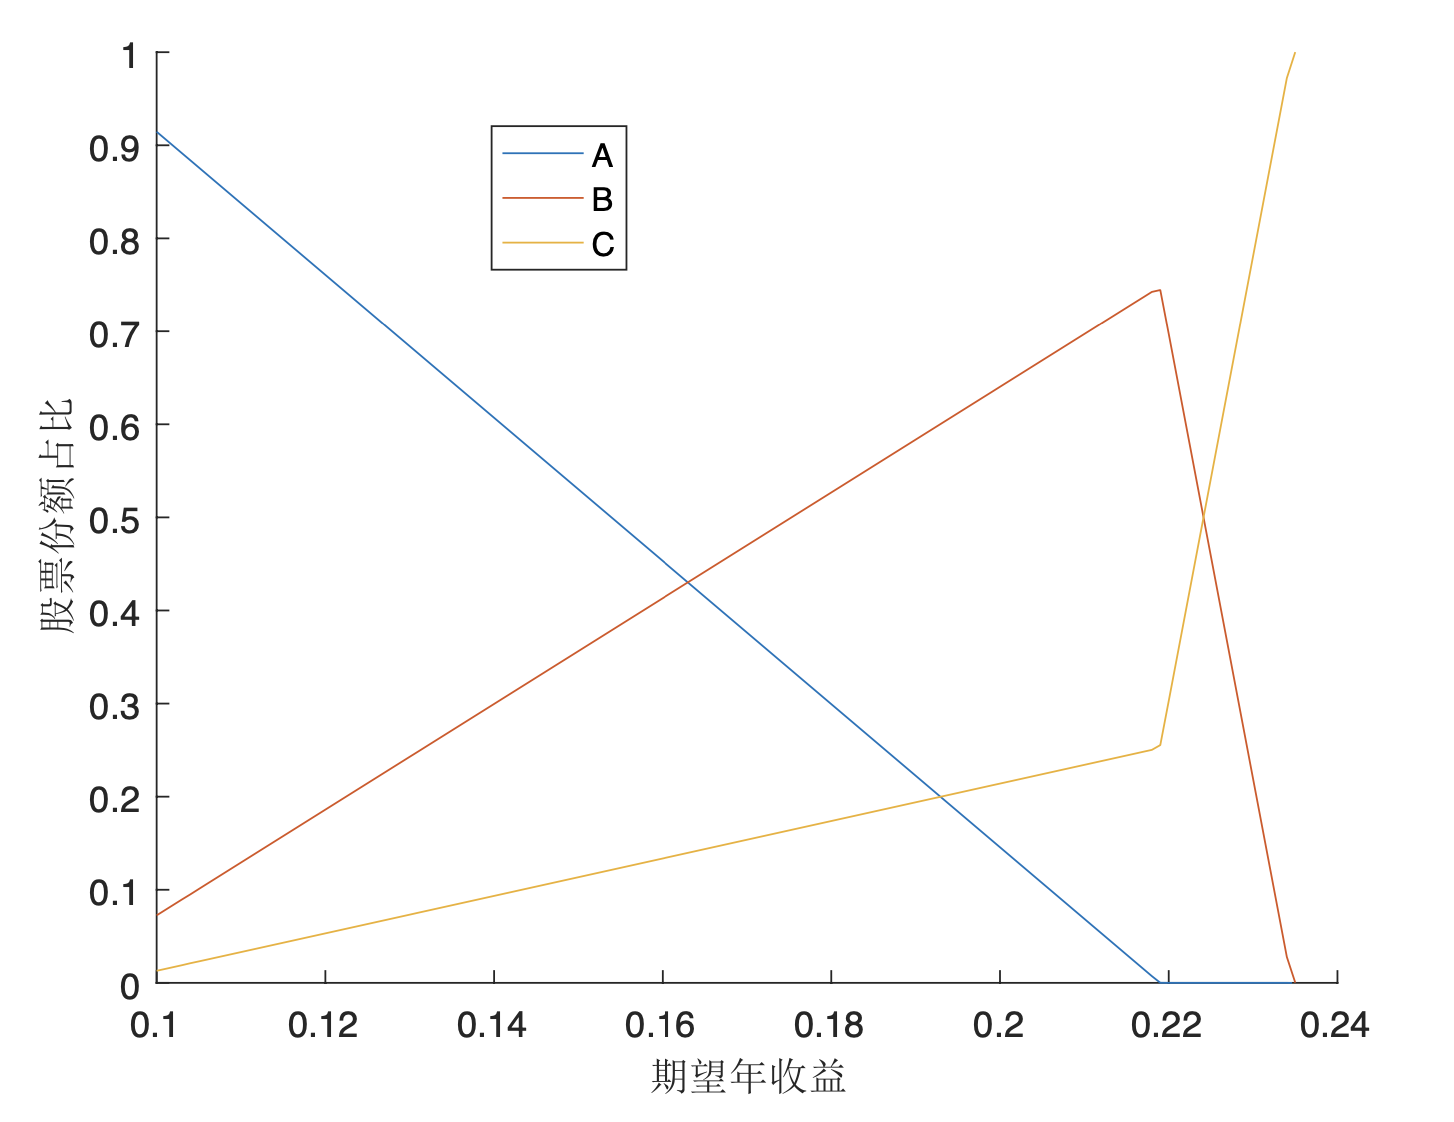
\includegraphics[width=0.6\textwidth]{pic3.png}
    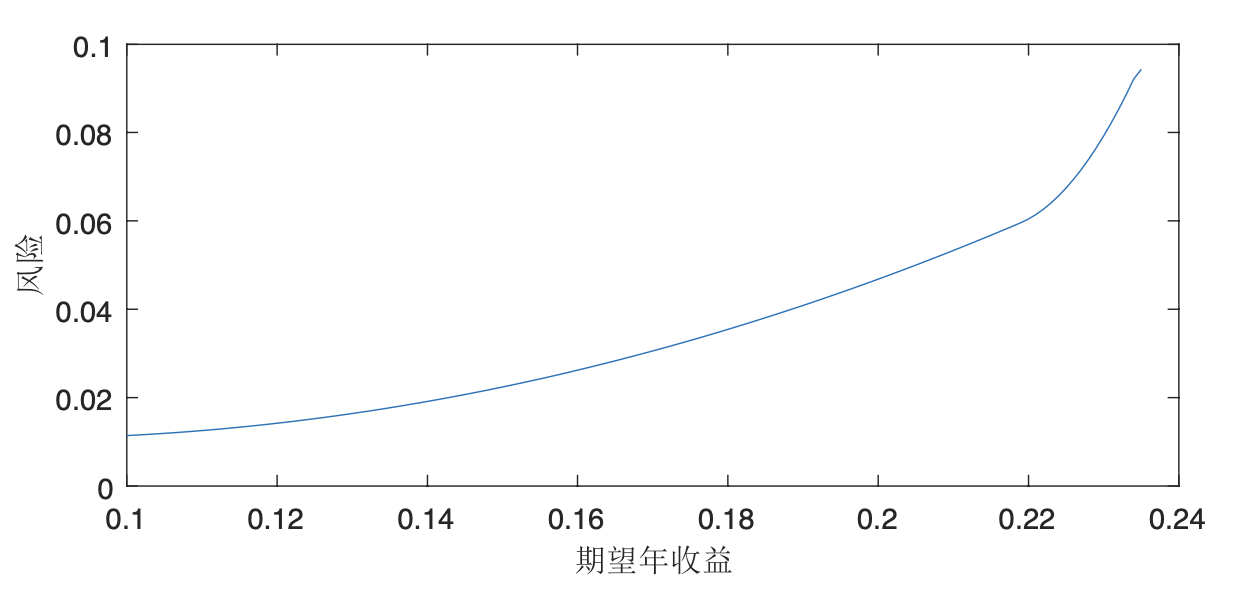
\includegraphics[width=0.6\textwidth]{pic4.png}

\end{figure}

可以看出,随着要求的期望年收益不断上升,对于股票 A 的购买应该逐步减少,当期望 达到 22\% 左右时应该完全不够买股票 A,最终随着期望年收益的进一步上升,全部都应该购买股票 C。根据风险图能够看出,随着期望收益的增高,其风险也越来愈高,这符合现实生 活的预期,收益越大,风险越大。投资需谨慎。

第 (2) 问:如果增加了国库券,LINGO 的求解的最优投资方案为:


$$a=0.087,b=0.43,c=0.14,d=0.34$$

相应的风险最小值为 0.021。相比不进行风险投资最小的风险值变小了。 对于第 (3) 问的新模型,LINGO 求解如下:

$$x_A=0.0266,y_A=0,x_B=0,y_B=0,x_C=0,y_C=0.0271$$

相应的风险最小值为 0.023。

\subsubsection{结论}

当期望年收益率达到 15\% 的时候,应该向 A 股票投资 53\%,向 B 股票投资 36\%, 向 C 股票投资 11\%。


当期望年利率在 10\% 到 100\% 变化时,投资组合和相应的风险变化如图 1和图 2所示。 相应的分析在上述章节。


如果考虑购买无风险的投资,则应该向 A 股票投资 9\%,向 B 股票投资 43\%,向 C 股 票投资 14\%,向无风险投资 34\%。


如果需要进行换手,则考虑买入 A 股票 2.66\%,卖出 C 股票 2.71\%(总额占比,即最终 持有的 A 股票为 52.66\%,B 股票为 35\%,C 股票为 12.29\%),能够满足最优解要求。


总结下来,期望越大,风险越高,投资的时候应该谨慎考虑可能发生的 各种问题,从历史数据学习经验,并利用数学模型进行合适求解,才能最优化我们的利益。


\section{实验总结}

通过这次的实验,我学会了 LINGO 软件的基本使用和编程技巧,并对非线性规划有了 更深的理解。希望在之后的课堂上老师能够当堂进行相关的技巧演示并给出题目的分步解答。

\end{document}